

\section{Filter-Based Shared Control}

\subsection{Maxwell Demon's Algorithm}

The Maxwell's Demon Algorithm (MDA) is a combined filter-controller computational unit that operates similar to the philosophical Maxwell's Demon from thermodynamics in that it accepts selected actions that meet a pre-defined criterion and disallows others. Specifically, it allows control actions that drive a system towards a pre-specified desired objective and disallows actions that drive the system away from that objective. The algorithm was originally proposed in \cite{MDA_Emmanouil} by Tzorakoleftherakis and Murphey, where the authors demonstrate that even noisy inputs, generated using i.e. a Gaussian distribution, can be a rich source of control authority if filtered in a meaningful manner. 

The algorithm was further developed by Fitzsimons et al. \cite{MDA_Katie} as a shared control paradigm for joint human-robot systems. In that work, authors show that MDA is able to improve task performance for technology-assisted tasks by simply rejecting ``wrong" user inputs (rather than actively assisting in task completion). In the study, 9 subjects attempt the task of inverting a simulated cart-pendulum with MDA-based feedback. They achieve better performance at the task when controlling the system with either an MDA-based software filter or MDA-based haptic feedback, providing initial results that MDA could be applied to design useful human-machine interfaces. 

In this work, we build on the idea of using MDA for shared control. We discriminate and evaluate two application scenarios and hence define two respective MDA modes: training and assistance. In training mode, if user actions are rejected, no control is applied to the system; in assistance mode, if user inputs are rejected, they are replaced with a controller-calculated action---this principle is illustrated in Fig.~\ref{fig: accept_reject_replace} on the example of a hand pushing a mass. 

In training mode, MDA improves task performance but allows for failure at the task without a rich enough input, making it well suited for robot-aided task training, where active engagement and failure are conducive to learning. Assistance mode, on the other hand, shows promise for being useful in allocating control of assistive devices, where safety and/or task success are of utmost importance. As mentioned above, we evaluate MDA in both modes---in training mode in Chapter~\ref{chapter: training}, and in assistance mode in Chapter~\ref{chapter: assistance}. 

\begin{figure}[h]
\centering
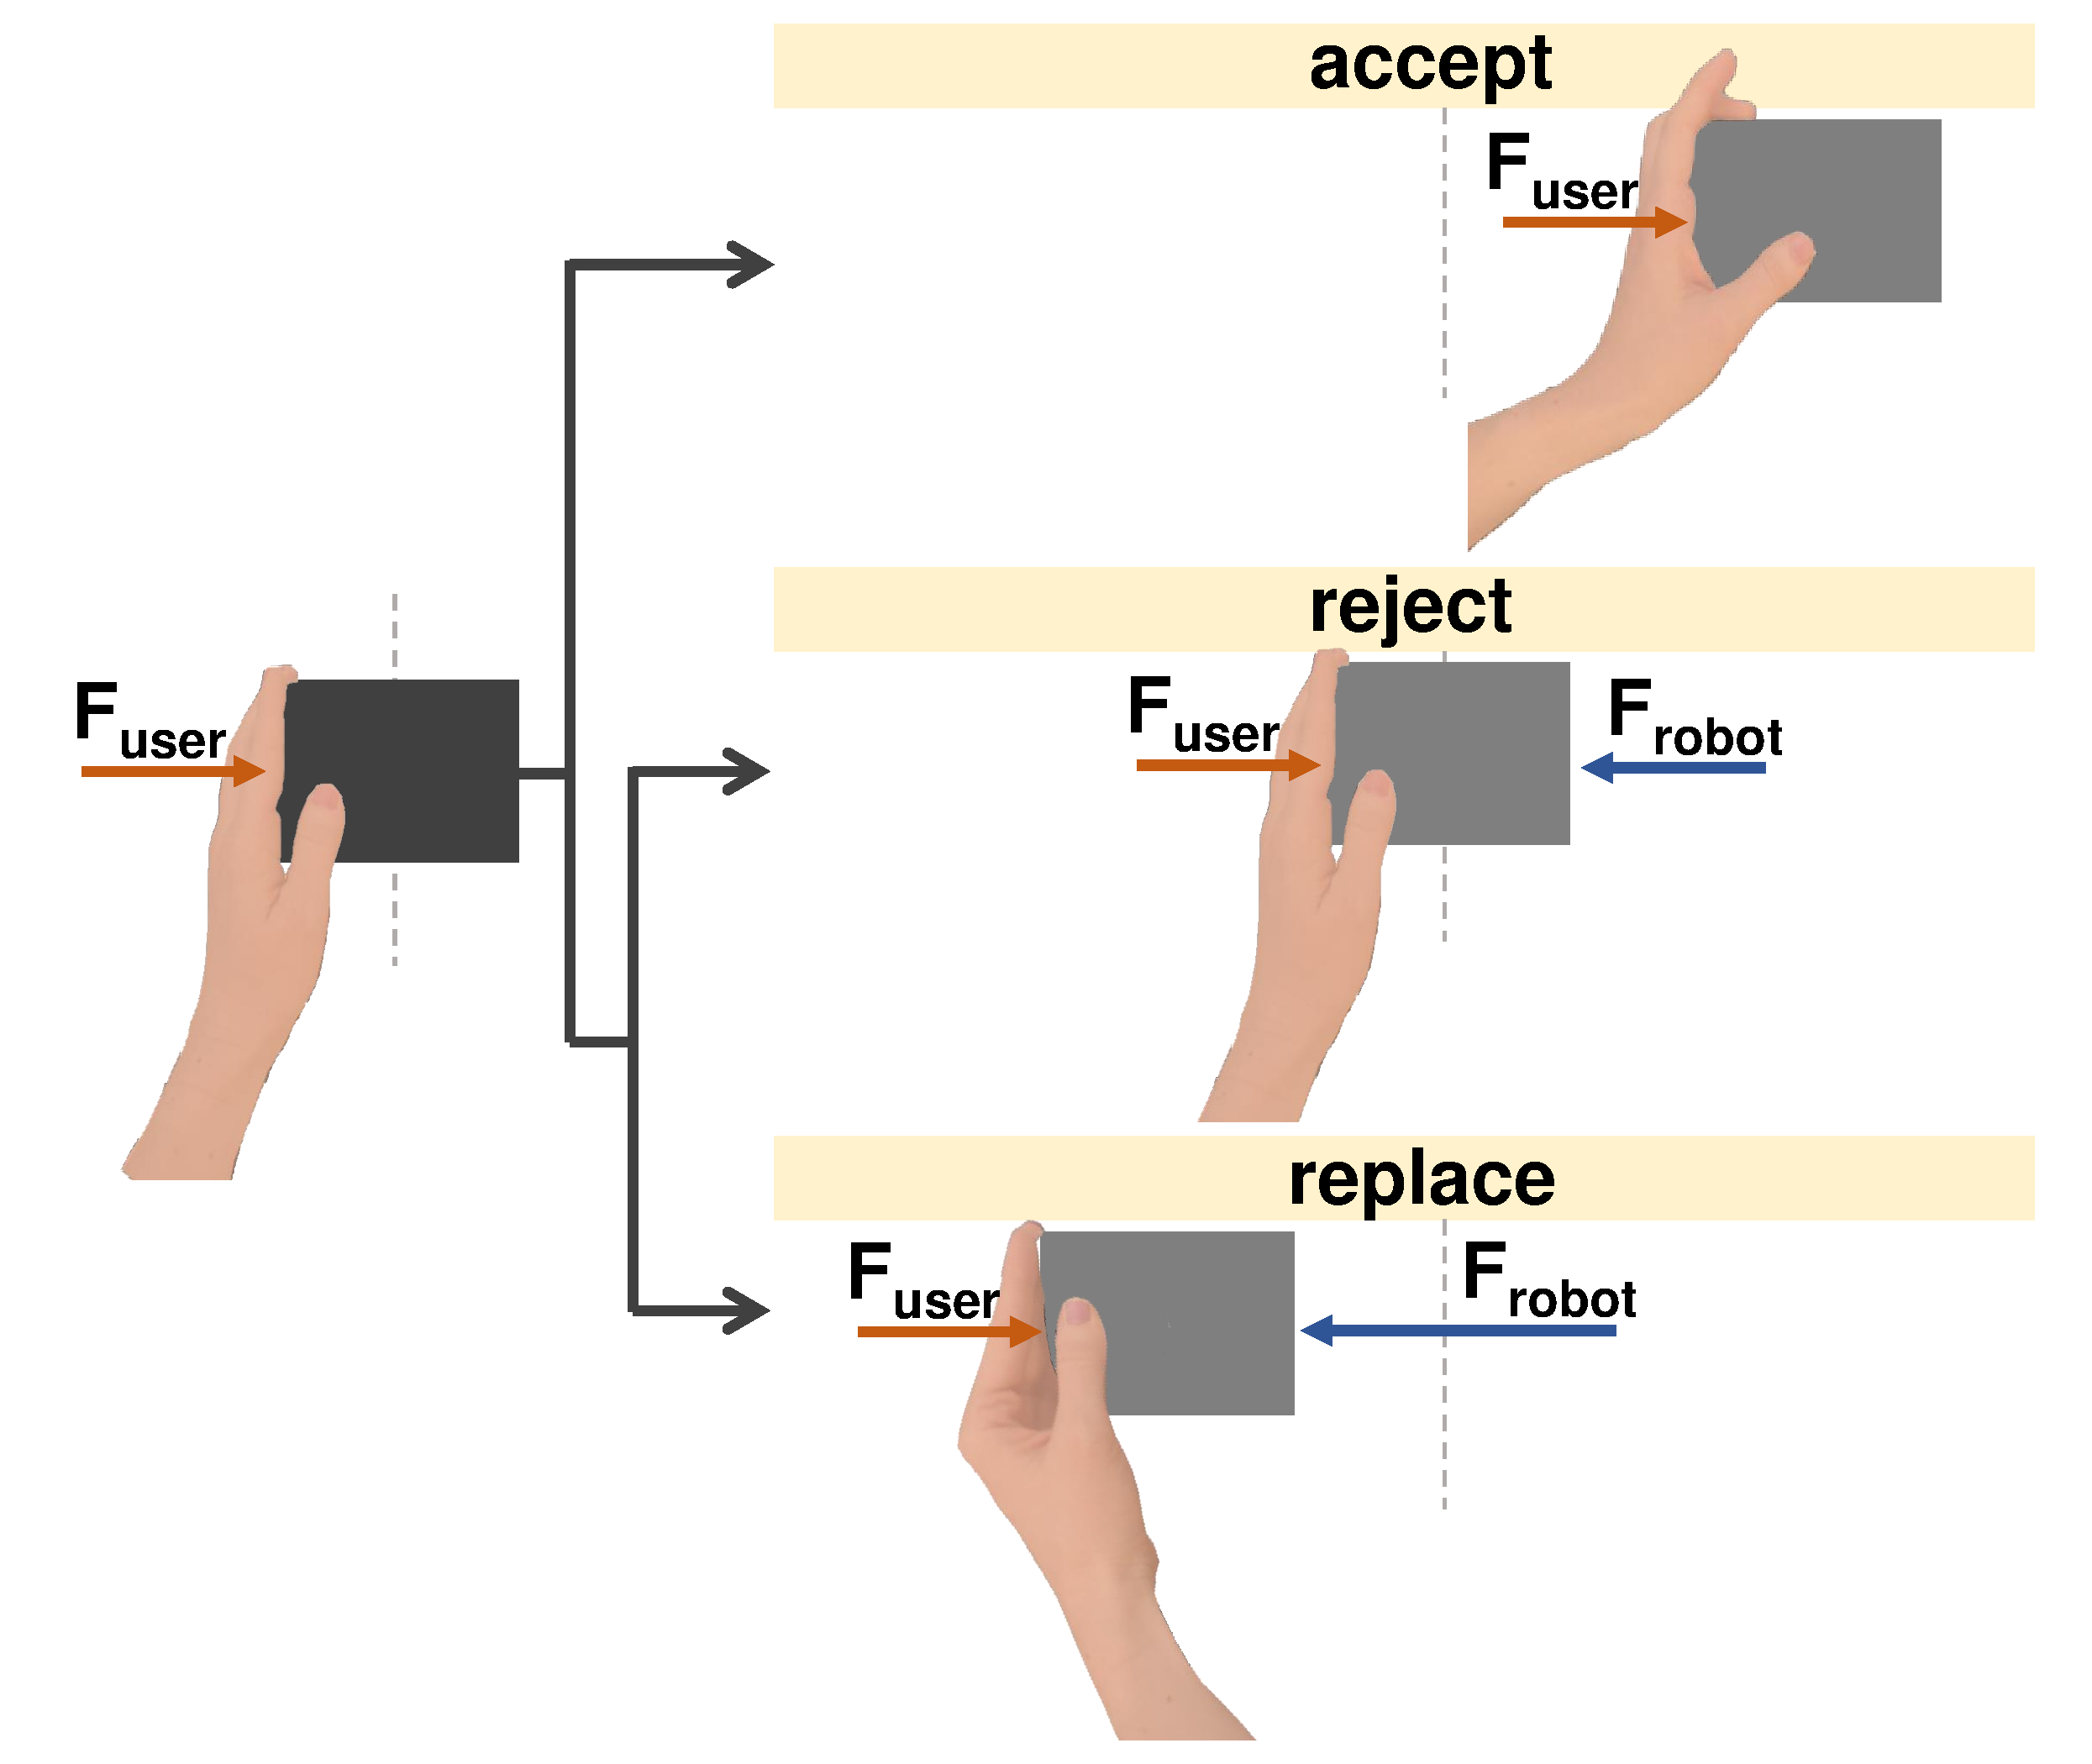
\includegraphics[width=0.7\columnwidth]{MDAconcept.pdf}
\caption{Filter-based robotic responses on the example of a hand pushing a mass. The robot filters user input by physically accepting, rejecting, or replacing it. When a user action is accepted, the robot admits the force. When a user action is not accepted, the robot either rejects it by applying an equal and opposite force or replaces it by applying a force, such that the net effect on the system is equal to the controller-calculated input. }
\label{fig: accept_reject_replace}
\end{figure}



\subsection{Mode Insertion Gradient (MIG) as a Criterion}
\label{criterion}

In shared control applications, a key part of the Maxwell's Demon Algorithm is the criterion used for evaluating user actions. In both \cite{MDA_Emmanouil} and \cite{MDA_Katie}, MDA was implemented with a criterion based on a direct comparison of user actions to the actions calculated by an optimal controller. In the studies presented here, we instead use the Mode Insertion Gradient (MIG) as an evaluation criterion of user inputs, which allows us to give users more flexibility in the way they approach a task. 

Usually, the MIG $ \frac{dJ}{d\lambda}$ is used, in mode scheduling problems, to determine the optimal time $\tau$ to insert control modes from a predetermined set ~\cite{egerstedt2006,modesched2012,vaseduvan_switchsys2010, alex_SAC, caldwell2016}. Here we use the mode insertion gradient,
\begin{equation}\label{mig}
    \frac{dJ}{d\lambda}(\tau)=\rho(\tau)^T \left[f(x(\tau),u_2(\tau))-f(x(\tau),u_1(\tau))\right],
\end{equation}
as a measure of the sensitivity of the cost to a change from the nominal control, $u_1$, to a particular user input, $u_2$. In (\ref{mig}), state $x$ is calculated using nominal control, $u_1$, and $\rho$ is the adjoint variable calculated from the nominal trajectory $x(t)$,
\begin{equation*}
    \dot \rho = -\nabla l_1(x)-D_xf(x,u_1)^T\rho,
\end{equation*}
where $l_1(x,t)$ is the incremental cost and $\rho(t_f)=\nabla m(x(t_f))$. Moreover, in the work presented here, we define the nominal control, $u_1$, to be equivalent to a null action ($u_1(t) = 0$), and we define $u_2$ with the piece-wise function below,
\[ u_2(t) =  \left\{
		\begin{array}{ll}
  			u_{user} & t\leq t_s \\
  			u_1 & t_s\leq t\leq T \\
		\end{array} 
\right. \]
where $t_s$ is the sampling time, $T$ is the time window over which we are evaluating system behavior, and $u_{user}$ is a user input recorded at current time $t$. It is worth noting that, in future work, $u_2$ could instead be defined by a combination of user input at current time $t$ and actions from an optimal controller over time $T$ into the future. This would add further flexibility to the criterion and give the user more control authority over the joint system, because any user action that could be corrected for by a future optimal action or sequence of optimal actions without destabilizing the system during the time window $T$ would be admitted.  

When using MIG as an evaluation criterion, we calculate the integral of the mode insertion gradient over a time window $T$ into the future
\begin{equation}\label{mig_int}
    \int_{t_{now}}^{t_{now}+T}\frac{dJ}{d\lambda}(t)\delta t,
\end{equation}
to evaluate the impact of user control $u_2$ on the system over time $T$. We show that, when negative, the integral indicates that $u_2$ is a descent direction over the entire time horizon, and thus can serve as the basis for evaluating the impact of a current user action on the evolution of a dynamic system over that time window into the future. Moreover, stability can be inferred if (\ref{mig_int}) satisfies a contractive constraint \cite{contractive, iSAC}. 

\noindent\begin{minipage}{\columnwidth}
\renewcommand\footnoterule{} 
\begin{algorithm}[H]
	\caption{A filter with MIG criterion.}\label{algo}
	\noindent\footnotetext{\noindent\normalsize *Note that the filter can be used with any model predictive controller (MPC) that can complete the task. Here a controller similar to the conjugate gradient descent method\cite{conjugate_gradient} was used.}
		    \\         
        Set sampling time $t_s$ and time horizon $T$. Set mode $m$ to either training $(T)$ or assistance $(A)$. Define objective function for filter and controller.
		\begin{algorithmic}[1]
			\While {$t_0 \leq t_f$}
			\State Infer user control vector $u_{user}$ from sensor data
			\State Simulate $x(t)$ and $\rho(t)$ in $[t_{now}, t_{now} + T]$ assuming \[ u =  \left\{
			\begin{array}{ll}
      			u_{user} & t\leq t_s \\
      			0 & t_s\leq t\leq T \\
			\end{array} 
			\right. \]
			\State Compute $\int \frac{dJ}{d\lambda}$
			\If {$ \int \frac{dJ}{d\lambda} \leq 0$}
			\State $u_{now} = u_{user}$
			\Else
			\If {$m=T$}
			\State Assign controller value
			$ u_{now} = 0 $
			\ElsIf {$m=A$}
			\State Calculate optimal control $u_{controller}$*
			\State Assign controller value 
			$ u_{now} = u_{controller} $
			\EndIf
			\EndIf
			\State Apply $u_{now}$ for $ t \in [t_{now}, t_{now}+t_s]$
			\EndWhile
		\end{algorithmic}	
	\end{algorithm}
	\renewcommand\footnoterule{}
\end{minipage}
\vspace{0.7cm}

In our experimental study, we utilize the MIG criterion in a filter-based shared control scheme. For an outline of the approach, refer to Algorithm \ref{algo}. 


\section{Simulated Users}
\label{section: simulated users}

%\begin{figure}[h]
%\begin{subfigure}{0.45\textwidth}
%\centering \captionsetup{width=0.9\linewidth}
%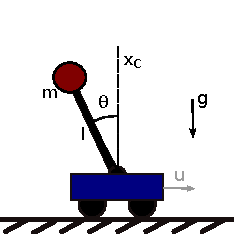
\includegraphics[width=\linewidth]{cart-pend.pdf}
%\caption{Subject Specific Trends}
%\end{subfigure}
%\begin{subfigure}{0.45\textwidth}
%\centering \captionsetup{width=0.9\linewidth}
%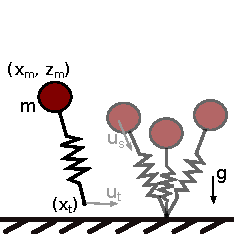
\includegraphics[width=\linewidth]{SLIP.pdf}
%\caption{Mean Across Subjects}
%\end{subfigure}
%\caption{\textbf{Percent of Accepted Actions} There are no discernible trends in Controller Engagement over time.}
%\end{figure}

\begin{figure}[h]
\centering \captionsetup{width=0.45\linewidth}
\begin{multicols}{2}
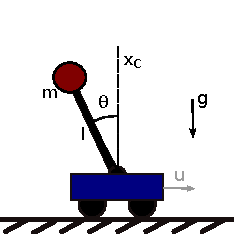
\includegraphics[width=0.9\columnwidth]{cart-pend.pdf}
\caption{The cart-pendulum system with state vector $x=[\theta, \dot{\theta}, x_c, \dot{x_c}]$ and horizontal acceleration of the cart as control input.}
\label{fig: cartpend-schematic}
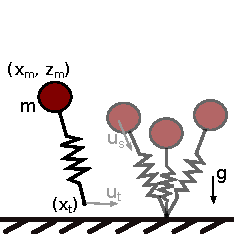
\includegraphics[width=0.9\columnwidth, keepaspectratio]{SLIP.pdf}
\caption{The SLIP model with state vector $x = [x_m, \dot{x}_m, z_m, \dot{z}_m, x_t]$ and control vector $u = [u_s,u_t]$, where $u_s$ is the leg thrust applied during stance and $u_t$ is the toe velocity control applied during flight.}
\label{fig: slip-schematic}
\end{multicols}
\end{figure}

To test the proposed algorithm in assistance mode, we run experiments with simulated users. We use Gaussian noise as well as a Model Predictive Controller (MPC) with differing objective functions to simulate users of varying skill levels. Specifically, an objective function defined as 
\begin{equation}
J = \frac{1}{2} \int_{t_o}^{t_f} \lVert x(t) - x_d(t)\rVert_{Q}^2 + \lVert u(t) \rVert_{R}^2 \delta t,
\end{equation}
with $Q \ge 0$ and $R \ge 0$ being metrics on state error and control effort and $x_d(t)$ being the desired trajectory is used in the simulated experiments. The systems and specific objective functions are described in the sections below. 


\subsection{Cart-Pendulum Task}

A cart-pendulum system as illustrated in Fig.~\ref{fig: cartpend-schematic} is one of the systems used. It has a state vector $x=[\theta, \dot{\theta}, x_c, \dot{x_c}]$ and a horizontal acceleration of the cart $u$ as control input. The task associated with this system is to invert the pendulum to its unstable equilibrium, where $\theta = 0$ and $\dot{\theta} = 0$. 

\begin{figure}[h]
	\begin{center}
		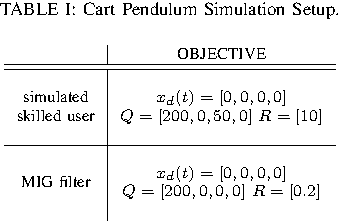
\includegraphics[width=0.6\columnwidth, keepaspectratio]{cp_table.pdf}\par
	\end{center}
\caption*{}
\vspace{-1.3cm}
\label{table_cp}
\end{figure}

To create the simulated skilled users, we utilize an MPC with objectives representing successful inversion strategies. An example objective includes inverting the cart-pendulum while minimizing energy and staying close to the origin---the exact function parameters are given in Table 1. To approximate an unskilled user, we generate noise input, using a Gaussian distribution within the saturation limits. While we made the above choices, there are other reasonable alternatives for representing simulated users.

In either case, we then filter user actions using a MIG-based algorithm with a high-level objective function also listed in Table 1. For the MIG filter, we choose to place a high weight only on the angle $\theta$. The goal is to emphasize the task of inversion while minimally limiting users' varying approach strategies.


\subsection{SLIP Hopper}

Another system used is the spring-loaded inverted pendulum. The SLIP is a hybrid, low-dimensional system that has been shown to be a reliable approximation of human running \cite{SLIP_for_running_nature} and is therefore used to model running dynamics in robotic locomotion \cite{SLIP_robot_evidence}. Here, a 2D SLIP model (Fig.~\ref{fig: slip-schematic}) is tested with a state vector described by $x = [x_m, \dot{x}_m, z_m, \dot{z}_m, x_t]$, where $x_m$ and $z_m$ are the coordinates of the mass, and $x_t$ is the coordinate of the toe, and a control vector described by $u = [u_s,u_t]$, where $u_s$ is the leg thrust applied during stance and $u_t$ is the toe velocity control applied during flight. Hybrid dynamics of the form
\begin{align*}
    f_{stance}= 
    \begin{pmatrix}
    \dot{x}_m \\
    \frac{(k(l_0-l_s)+u_s)(x_m-x_t)}{ml_s} \\
    \dot{z}_m \\
    \frac{(k(l_0-l_s)+u_s)z_m}{ml_s} - g \\
    0
    \end{pmatrix}
\end{align*}
and $f_{flight} = (\dot{x}_m,0,\dot{z}_m,-g,\dot{x}_m+u_t) $
are used. Parameters $k$, $l_0$, and $m$ describe the SLIP model spring constant, resting spring length, and mass, respectively. All parameters were given a value of 1 in our simulations. 

To determine switches between stance and flight modes, a guard equation $\phi(x)$ is employed
\begin{equation*}
    \phi_{stance \rightarrow flight}(x) = \phi_{flight \rightarrow stance}(x) = x_m - \frac{l_0}{l_s}z_m
\end{equation*}
with $l_s$ being the leg length during stance
\begin{equation*}
    l_s=\sqrt{(x_m-x_t)^2+z_m^2}.
\end{equation*}

In the experiments, we again use input from simulated users of different skill level, which we generate using MPC with objective functions outlined in Table 2. We approximate an unskilled user using Gaussian noise; a low-skill user using MPC with a height objective lower than the spring length, which causes the SLIP to fall if simulated without assistance; and a skilled user using MPC with a feasible objective such that the controller can achieve forward motion without assistance. 

\begin{figure}[h]
	\begin{center}
		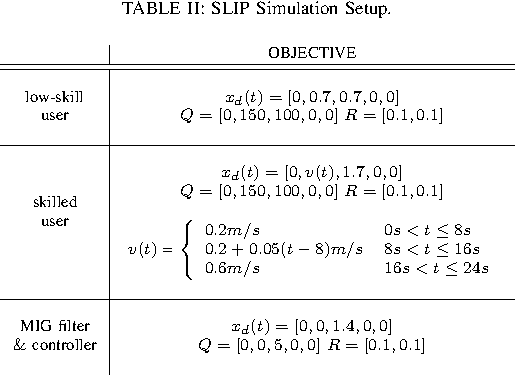
\includegraphics[width=0.6\columnwidth, keepaspectratio]{SLIP_table2.pdf}\par
	\end{center}
\label{table_slip}
\end{figure}

Here, the MIG-based filter uses a high-level objective function defining the height of the center of mass $z_m$, also listed in Table 2. The goal is to emphasize the safe upright orientation of the SLIP hopper while minimally limiting its movements and velocity in the $x$-direction.


\section{Human Subject Experiments}
\label{section: human experiments}

In addition to testing simulated users, we conducted a human subject study, where we implemented and tested the proposed shared control paradigm in the form of a mechanical filter. Subjects used an upper limb robotic platform as an interface to control a simulated cart-pendulum system. During experimental trials, users were instructed to invert the pendulum to its unstable equilibrium and keep it there for as long as possible. User input was inferred from a force sensor at the robot's end-effector and was continually evaluated at 100Hz. During trials when the filter was engaged, user actions were either accepted or rejected based on the criterion described in Section ~\ref{criterion}. 


\subsection{Experimental Platform}

All human subject data was collected using the robotic platform shown in Fig.~\ref{nact3d}. The device is a powerful haptic admittance-controlled robot that can be used to render virtual objects, forces, or perturbations in three degrees of freedom. It is similar to the robotic platform used in \cite{ellis2016} and \cite{stienen2011} to provide a means to modulate limb weight support during reaching and to quantify upper limb motor impairments in stroke survivors.

\begin{figure}[h]
\centering
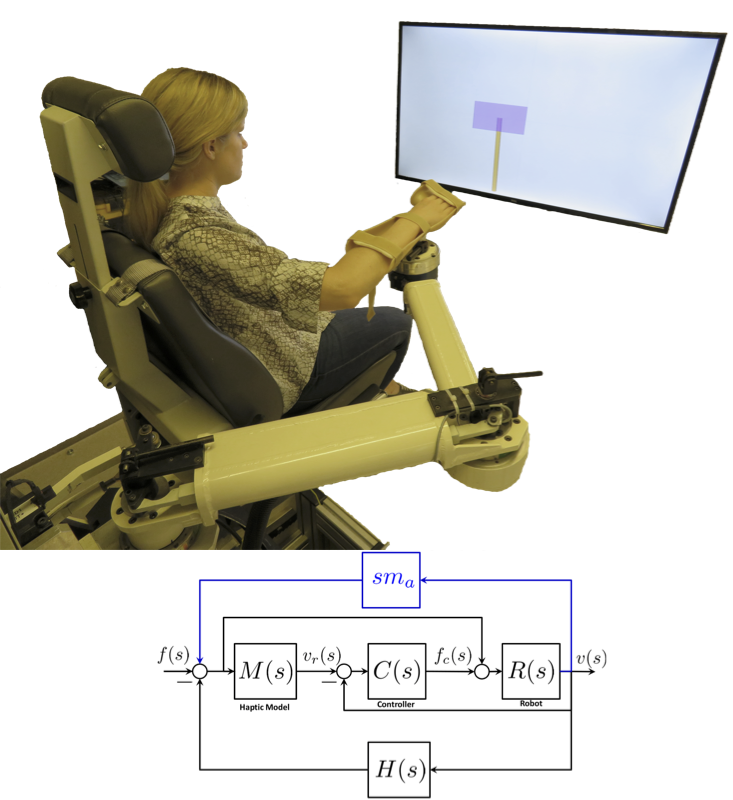
\includegraphics[width=0.7\columnwidth]{NACT-userview-small.png}
\caption{(top) Upper limb robotic platform used during experiments. (bottom) The platform provides haptic feedback to simulate a specified inertial model via an admittance control scheme. A voluntary force $f(s)$ is measured by a force-torque sensor at the end-effector and passed through a model $M(s)$ that determines velocity $v_r(s)$ at which the robot should move. The reference velocity is tracked by the low level velocity controls, $C(s)$, of each motor drive. In addition to a force input, the user delivers involuntary impedance forces due to movement, given by dynamics $H(s)$. Acceleration information is fed back as a pseudo-force $sm_a$ for extra inertia reduction of the system.}
\label{nact3d}
\end{figure}

During the experiment, each subject was seated in a Biodex chair with their arm secured in a forearm-wrist-hand orthosis. The orthosis could rotate passively, and the device could move its end-effector within a workspace defined both by its design limits and limits set by the investigators. At the point where the orthosis was mounted, a force-torque sensor measured subject input, which was then fed back to the admittance controller. In our experiments, the device was set up to physically support the upper limb of the participant in the z-direction while allowing them to move freely on the x-y plane. 

During testing, a display provided real-time visual state feedback to the user about the cart-pendulum system they were attempting to invert. High stiffness virtual springs in the haptic model were used to restrict user motion to a horizontal plane corresponding to the path of the cart in the virtual display. When user inputs were accepted, the control scheme behaved as described in Fig.~\ref{nact3d} and the end-effector motion changed according to the applied force. When user inputs were rejected, the measured user input $f(s)$ was ignored in the control scheme, such that the robot continued to move under its predefined dynamics as if no force had been applied by the user.

\subsection{Experimental Protocol} 

Twenty-eight subjects (9 males and 19 females) consented to participate in this study.\footnote{This study protocol was approved by the Institutional Review Board and all participants signed an informed consent form.} All subjects completed three sets of thirty 30-second trials with short breaks between sets. Each trial consisted of the subject attempting to invert a simulated cart-pendulum system, using cart acceleration as input. At the beginning of each session, the system and task was demonstrated to the subject using a video of a sample task completion. Subjects were instructed to attempt to swing up the simulated pendulum to the upward unstable equilibrium and balance it there for as long as possible. Subjects were instructed to continue to try to do this until the 30 seconds were over even if they succeeded at balancing near the equilibrium at some point throughout the trial.

Upon enrollment, subjects were randomly placed into either a control ($n=10$) or training group ($n=18$). During the second set, feedback in the form of a filter was engaged for the training group, while the control group completed each of the three sets without any feedback. Again, each user did three sets of thirty trials: set 1 (both groups: no feedback), set 2 (control: no feedback, training: feedback in the form of a mechanical filter), set 3 (both groups: no feedback). The experimental protocol is illustrated in Fig.~\ref{fig: exp_protocol}.

\begin{figure}[t]
\centering
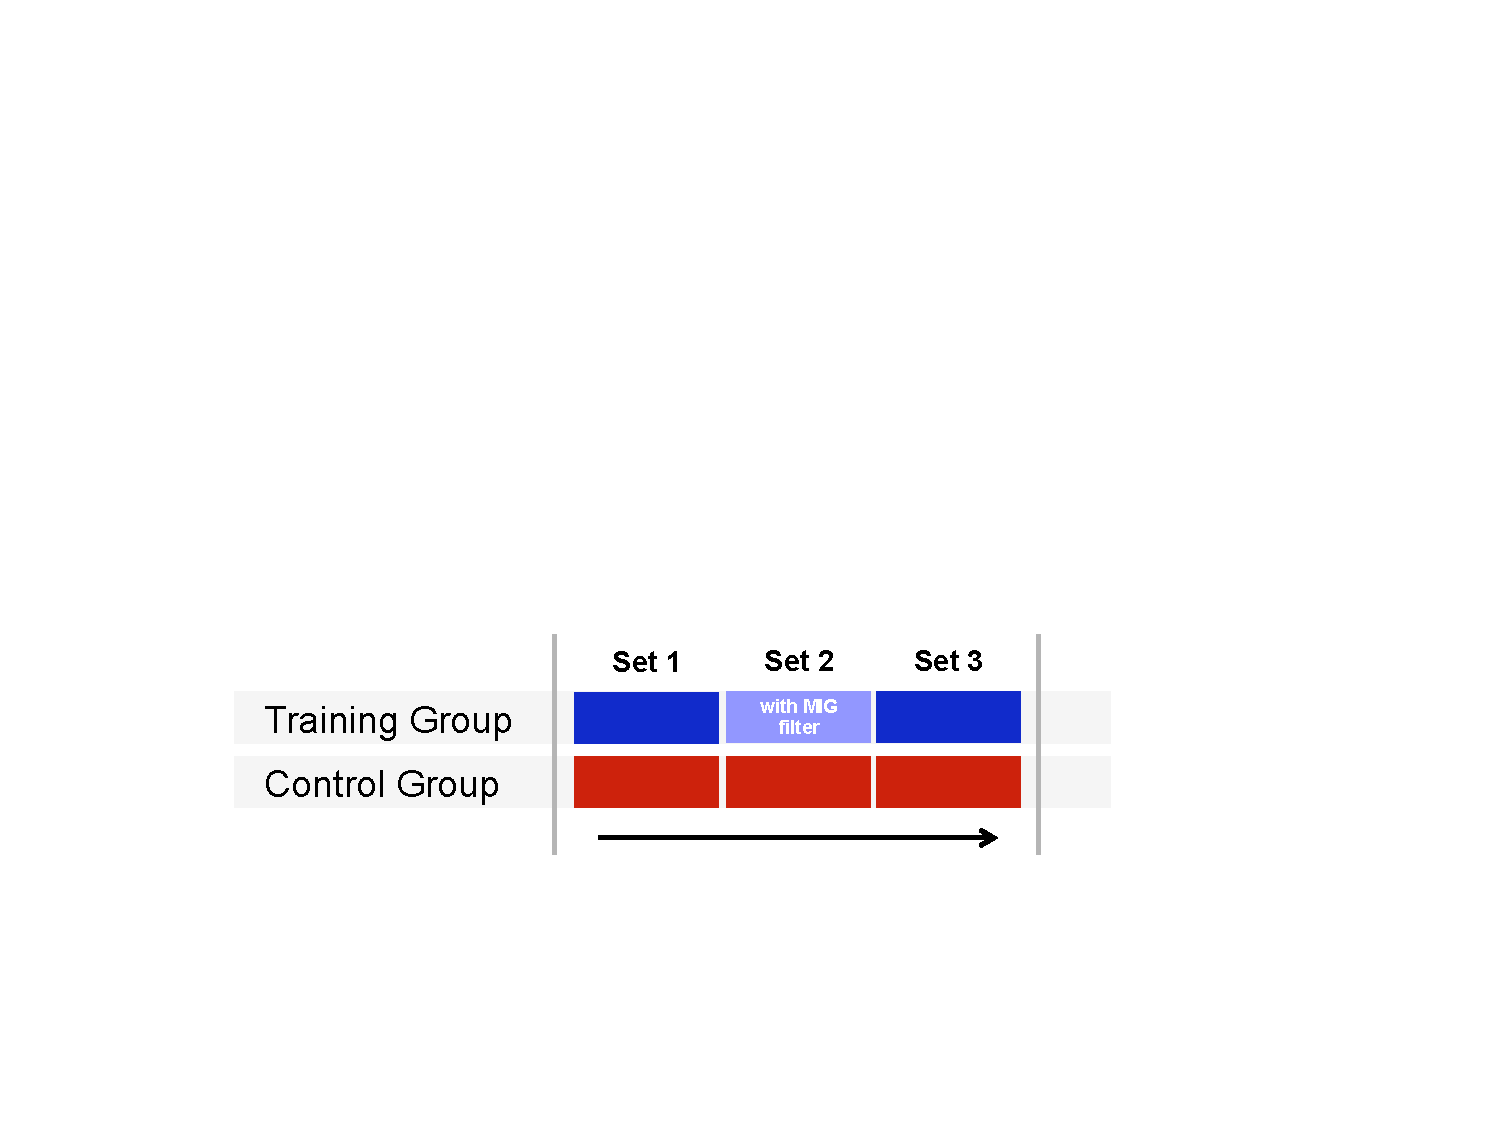
\includegraphics[width=0.7\columnwidth]{Exp_Protocol_MIG.pdf}
\caption{Experimental Protocol. Upon enrollment, subjects were randomly placed into either a control ($n=10$) or training group ($n=18$). Each session consisted of three sets of thirty trials (each block above represents one such set). In set 1, both groups received no feedback, in set 2 the control group trained without feedback while the training group trained with feedback in the form of a mechanical filter, and in set 3 both groups attempted the task again with no feedback.}
\label{fig: exp_protocol}
\end{figure}



\subsection{Performance Measures}\label{metrics}

Several measures were calculated to quantify user performance in individual trials. Specifically, time to success, balance time, and error were calculated for all trials and subsequently each trial was classified as successful or unsuccessful. 

A trial was considered successful when a subject reached an angle of $\pm0.4$~rad and angular velocity of $\pm0.75$~rad/s for at least 2 seconds. This success definition was used to determine the success rate and time to success of the users in each set. In addition, if a subject was successful, the total time spent at an angle of $\pm0.4$~rad and angular velocity of $\pm0.75$~rad/s 
\begin{figure}[!h]
\begin{center}
  	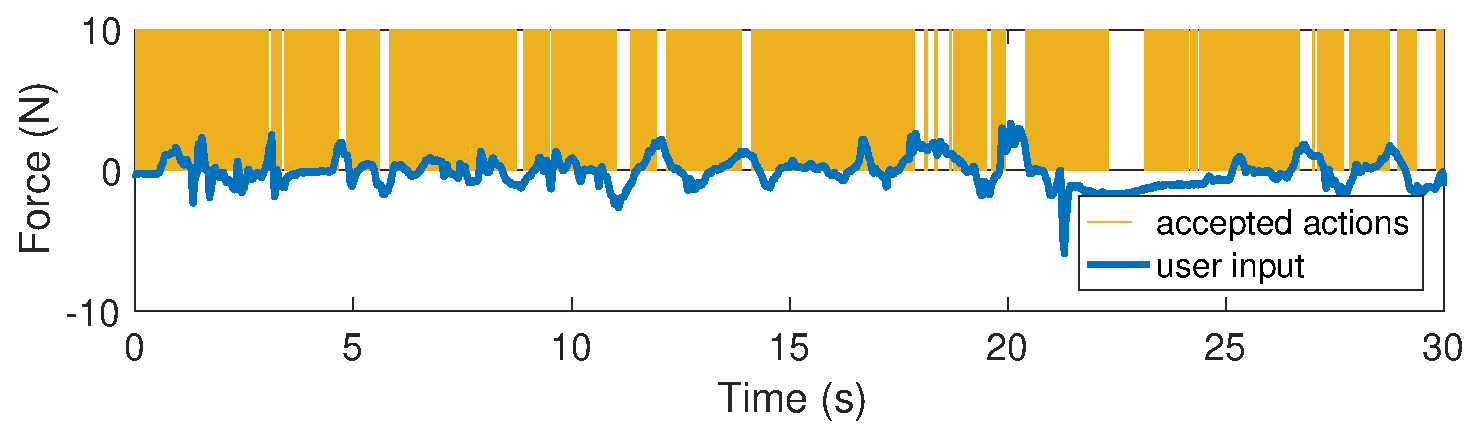
\includegraphics[width=1\columnwidth, keepaspectratio]{ie_good_user_input.eps}
  	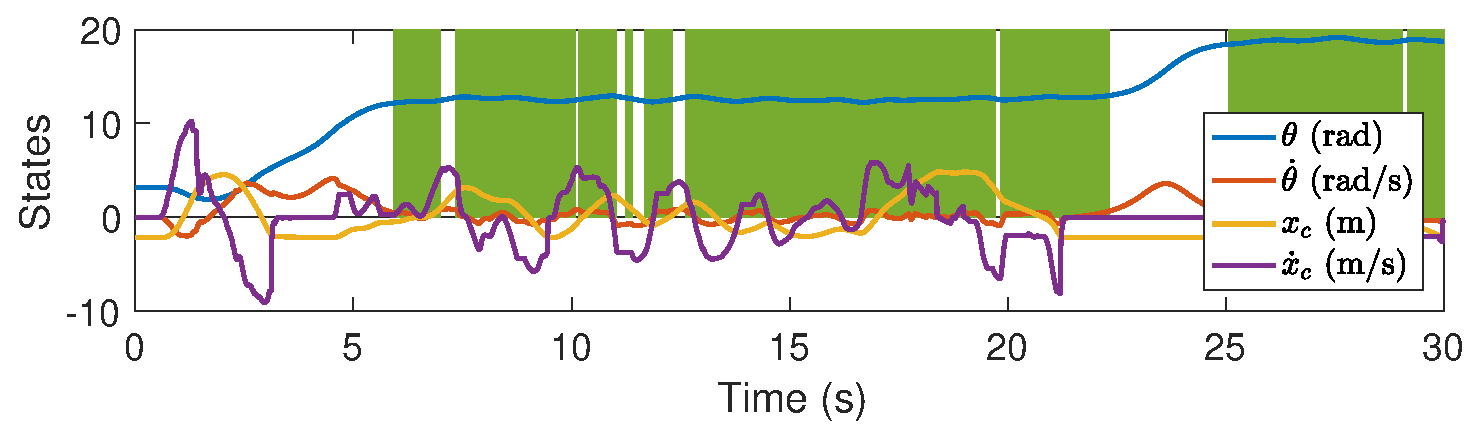
\includegraphics[width=1\columnwidth, keepaspectratio]{ie_good_user_states.eps}
\end{center}
\caption{Example trial data from study. (top) User force input with an indication of allowed actions in yellow. (bottom) System evolution with green highlighting of the time during which success was recorded. Note: Angle wrapping was not used on $\theta$ in the plot above, but it was used in the calculation of all performance measures. }
\label{fig: example_user}
\end{figure}
was recorded as the balance time. Note that when users were successful multiple times in the same trial, time spent in the balance region was cumulative. Lastly, an RMS error of each trajectory generated by the users was calculated with respect to the desired position in an inverted unstable equilibrium (zero-vector of the states). RMS error was normalized by the RMS error of a constant trajectory at the stable equilibrium, equivalent to the error of the user not moving from the initial conditions. 

A percent of rejected actions (PRA) was also recorded. PRA measured the fraction of user inputs that were rejected up to the time of a successful inversion, where we define an action to be a non-zero user input. 

Data from an example trial is visible in Fig.~\ref{fig: example_user}. In this case the trial was successful, with time to success = 8.3s, balance time = 19.7s, and RMS error = 0.57. The PRA was $13\%$.

